\documentclass{article}



\usepackage{arxiv}

\usepackage[utf8]{inputenc} % allow utf-8 input
\usepackage[T1]{fontenc}    % use 8-bit T1 fonts
\usepackage{hyperref}       % hyperlinks
\usepackage{url}            % simple URL typesetting
\usepackage{booktabs}       % professional-quality tables
\usepackage{amsfonts}       % blackboard math symbols
\usepackage{nicefrac}       % compact symbols for 1/2, etc.
\usepackage{microtype}      % microtypography
\usepackage{lipsum}		% Can be removed after putting your text content
\usepackage{graphicx}
\usepackage{natbib}
\usepackage{doi}

\usepackage[dvipsnames]{xcolor}
\newcommand{\andy}[1]{\textcolor{blue}{\emph{#1}}}

\title{Could mass eccentricity explain the formation of orbits in wind turbines?}

%\date{September 9, 1985}	% Here you can change the date presented in the paper title
%\date{} 					% Or removing it

\author{ \href{https://orcid.org/0000-0000-0000-0000}{
\includegraphics[scale=0.06]{orcid.pdf}\hspace{1mm} Aljoscha Sander}\thanks{Use footnote for providing further information about author (webpage, alternative address)---\emph{not} for acknowledging funding agencies.} \\
	Energy and Sustainability Research Institute Groningen\\
	University of Groningen\\
	Groningen, the Netherlands \\
	\texttt{aljoscha.sander@rug.nl} \\
	%% examples of more authors
	\And
	\href{https://orcid.org/0000-0000-0000-0000}{
\includegraphics[scale=0.06]{orcid.pdf}\hspace{1mm} Andreas Haselsteiner} \\
	\texttt{a.haselsteiner@uni-bremen.de} \\
	\And
	Bas Holman \\
	\texttt{b.holman@outlook.com}\\
	%% Address \\
	%% \texttt{email} \\
	%% \And
	%% Coauthor \\
	%% Affiliation \\
	%% Address \\
	%% \texttt{email} \\
	%% \And
	%% Coauthor \\
	%% Affiliation \\
	%% Address \\
	%% \texttt{email} \\
}

% Uncomment to remove the date
%\date{}

% Uncomment to override  the `A preprint' in the header
%\renewcommand{\headeright}{Technical Report}
%\renewcommand{\undertitle}{Technical Report}
\renewcommand{\shorttitle}{Mass eccentricity in offshore wind turbines}

%%% Add PDF metadata to help others organize their library
%%% Once the PDF is generated, you can check the metadata with
%%% $ pdfinfo template.pdf
\hypersetup{
pdftitle={Could mass eccentricity explain the formation of orbits in wind turbines?},
pdfsubject={},
pdfauthor={Aljoscha Sander, Andreas Haselsteiner, Bas Holman},
pdfkeywords={First keyword, Second keyword, More},
}

\begin{document}
\maketitle

\begin{abstract}
	blablabla
\end{abstract}


% keywords can be removed
\keywords{First keyword \and Second keyword \and More}


\section{Introduction}
\label{sec:introduction}

Offshore wind is growing continuously and is on its way to become one of the pillars of green energy. Recent cost reductions in offshore wind (29 \%) have mostly been due to increasing turbine size \citep{irenaRenewablePowerGeneration2020}. Increasing turbine size and numbers, however, leads to increasing difficulties during installation: Specialized vessels are needed and are in short supply and larger components are more difficult to handle and require more space on an installation vessel. Today, most turbines are installed component by component, including the blades, a process generally referred to as single blade installation \citep{jiangInstallationOffshoreWind2021}. Blades are installed utilizing a specialized tool, usually referred to as an installation yoke, that securely fastens the blade during craning operations. Once the blade reaches hub height, a guiding pin is used to land the blade's bolts in the corresponding holes in the flange. During this operation, relative motion between the blade root and the rotor hub greatly inhibits the secure landing of the blade in the rotor's flange. As these relative motions are driven by environmental loading on both the turbine and the blade, they are difficult to understand and even more so: to predict. 
In a measurement campaign during the installation of the offshore wind farm \textit{Trianel Windpark Borkum II} of the coast of Germany in the German Bight, the kinematics of blades and partially installed turbines was investigated \citep{sanderRelativeMotionSingle2020,  sanderMONITORINGOFFSHOREWIND2020, sanderOscillationsOffshoreWind2020}. These measurements revealed, that the partially installed turbines were displaying intricate patterns of motions - orbits - during single blade installation. A two-minute orbit captured during the installation of the wind park \textit{Trianel Windpark Borkum II} is shown in \autoref{fig:orbit}. These orbits show that amplitude and direction of tower top motion may occur swiftly and with large rates of change. It stands to reason that these orbits in turn influence the installation of blades and may even be responsible for an increase in installation difficulty.

\begin{figure}[ht!]
    \centering
    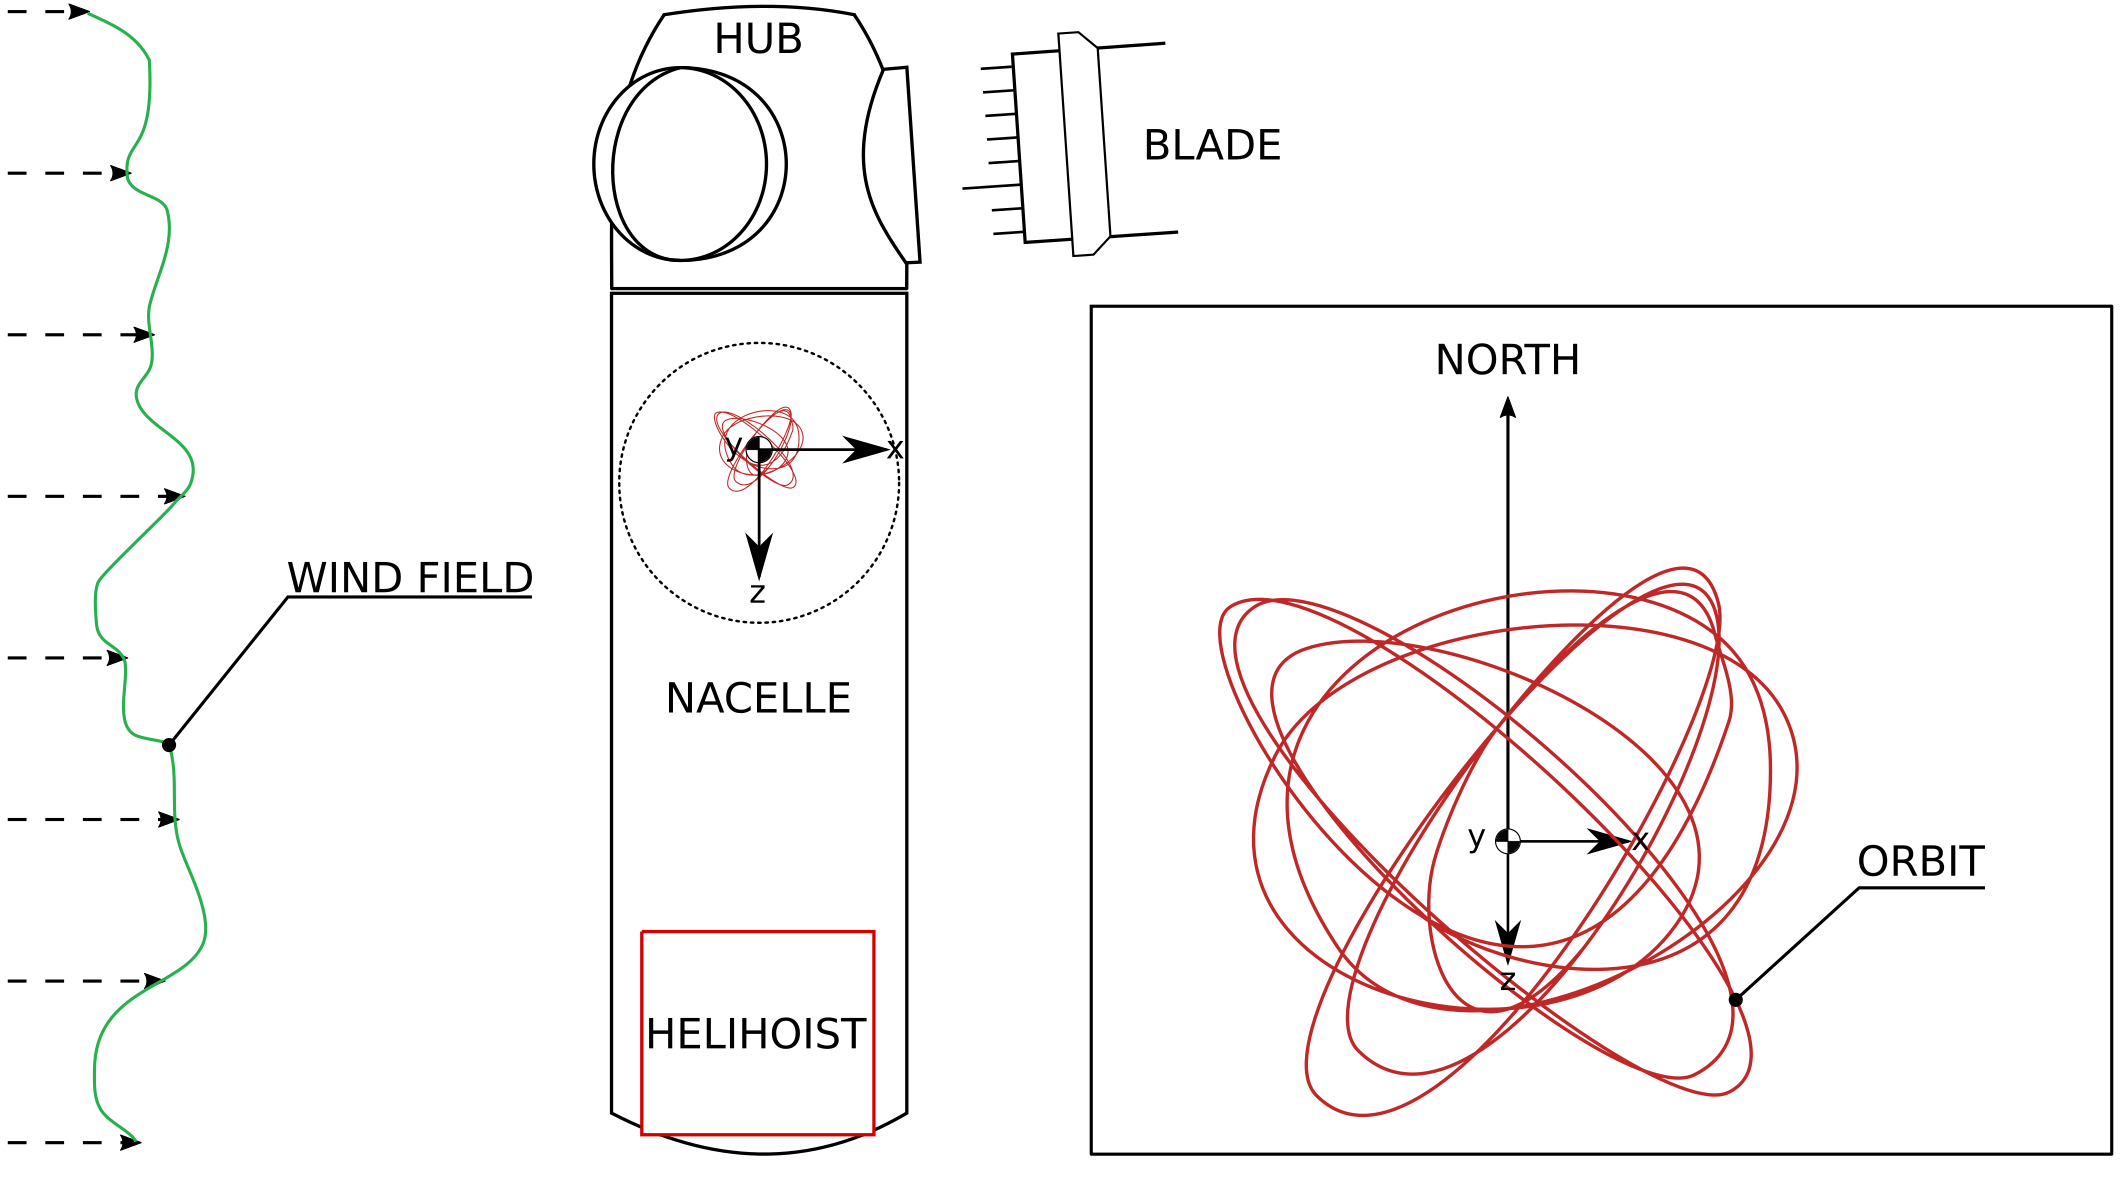
\includegraphics[width=0.7\linewidth]{manuscript/figures/installation_alt2.png}
    \caption{Formation of orbits as observed during the installation of the offshore wind park \textit{Trianel Windpark Borkum II}. Note: the orbits are not to scale to enhance visibility.}
    \label{fig:orbit}
\end{figure}

Several mechanisms may lead to the formation of orbits in offshore wind turbines. In this paper, we present a coupling mechanism that leads to the formation of orbits. 

In this paper, we focus on one specific state of an offshore wind turbine during installation: the hammerhead configuration. In this configuration, the foundation, transition piece, tower, and nacelle have already been installed, and the next installation step would be the installation of the first blade. In this configuration, the turbine is top heavy and, due to the nacelle's and rotor's weight, also nose-heavy. In the case of the turbines installed at \textit{Trianel Windpark Borkum II}, the centre of gravity of the nacelle is approximately 0.25 m shifted towards the rotor with respect to the tower axis. \autoref{fig:loading} depicts the hammerhead configuration as well as the simplified mechanical system derived to investigate the behaviour of partially installed turbines during installation. 

\begin{figure}[ht!]
    \centering
    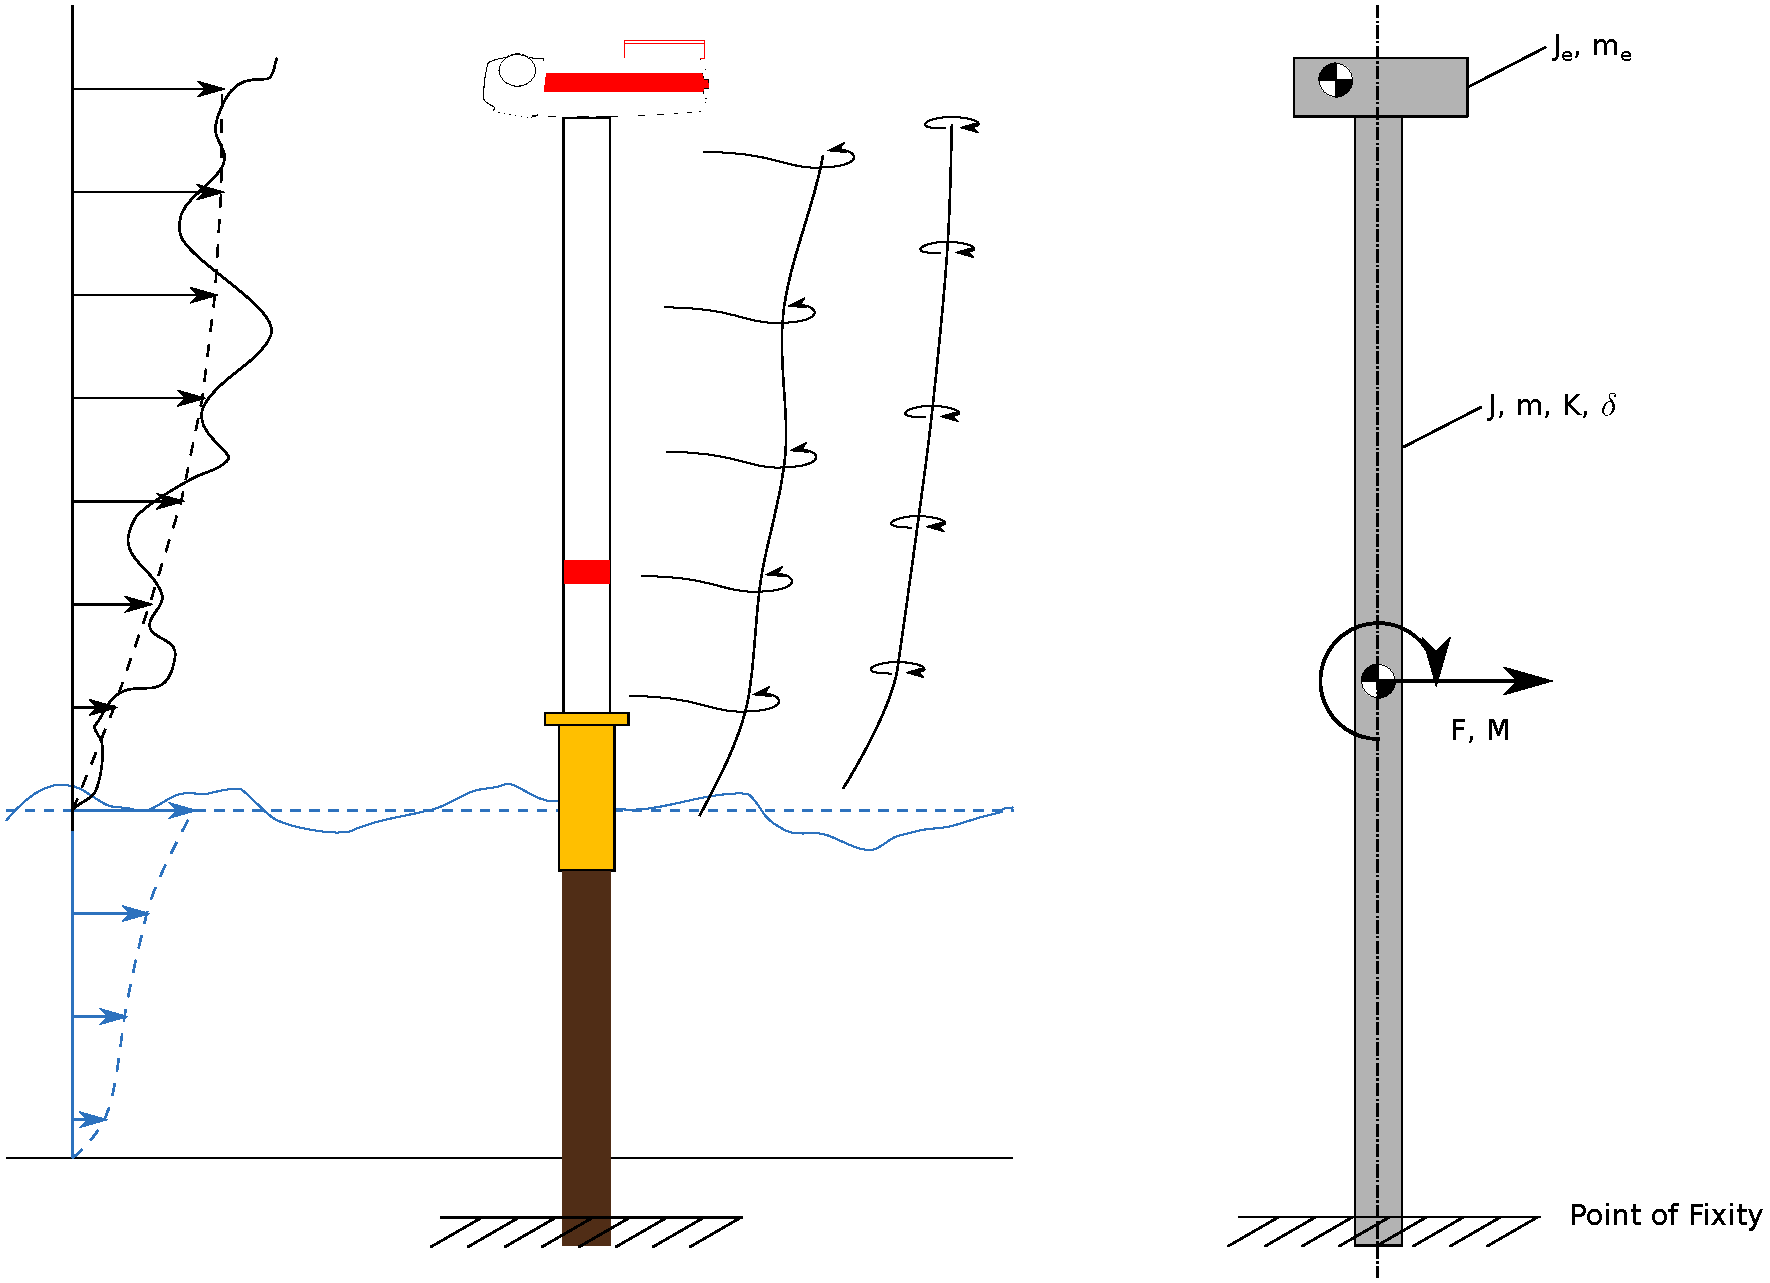
\includegraphics[width=0.7\linewidth]{manuscript/figures/loading_3.pdf}
    \caption{Hammerhead configuration (left) and simplified mechanical model of the hammerhead configuration (right).}
    \label{fig:loading}
\end{figure}

This system represents a cantilevered beam with an eccentric mass at the free end. We hypothesize that the inertia of the eccentric mass leads to torsion of the cantilevered beam if the tower vibrates transversally. Twisting the tower has two effects: a) the circular motion of the eccentric mass has a component perpendicular to the initial direction of motion, and thus momentum from that circular motion transfers into the perpendicular direction. b) twisting the tower leads to a torsional oscillation of the eccentric mass around the tower axis. The torsional motion of the eccentric mass in illustrated in \autoref{fig:kinematics}.

\begin{figure}[ht!]
    \centering
    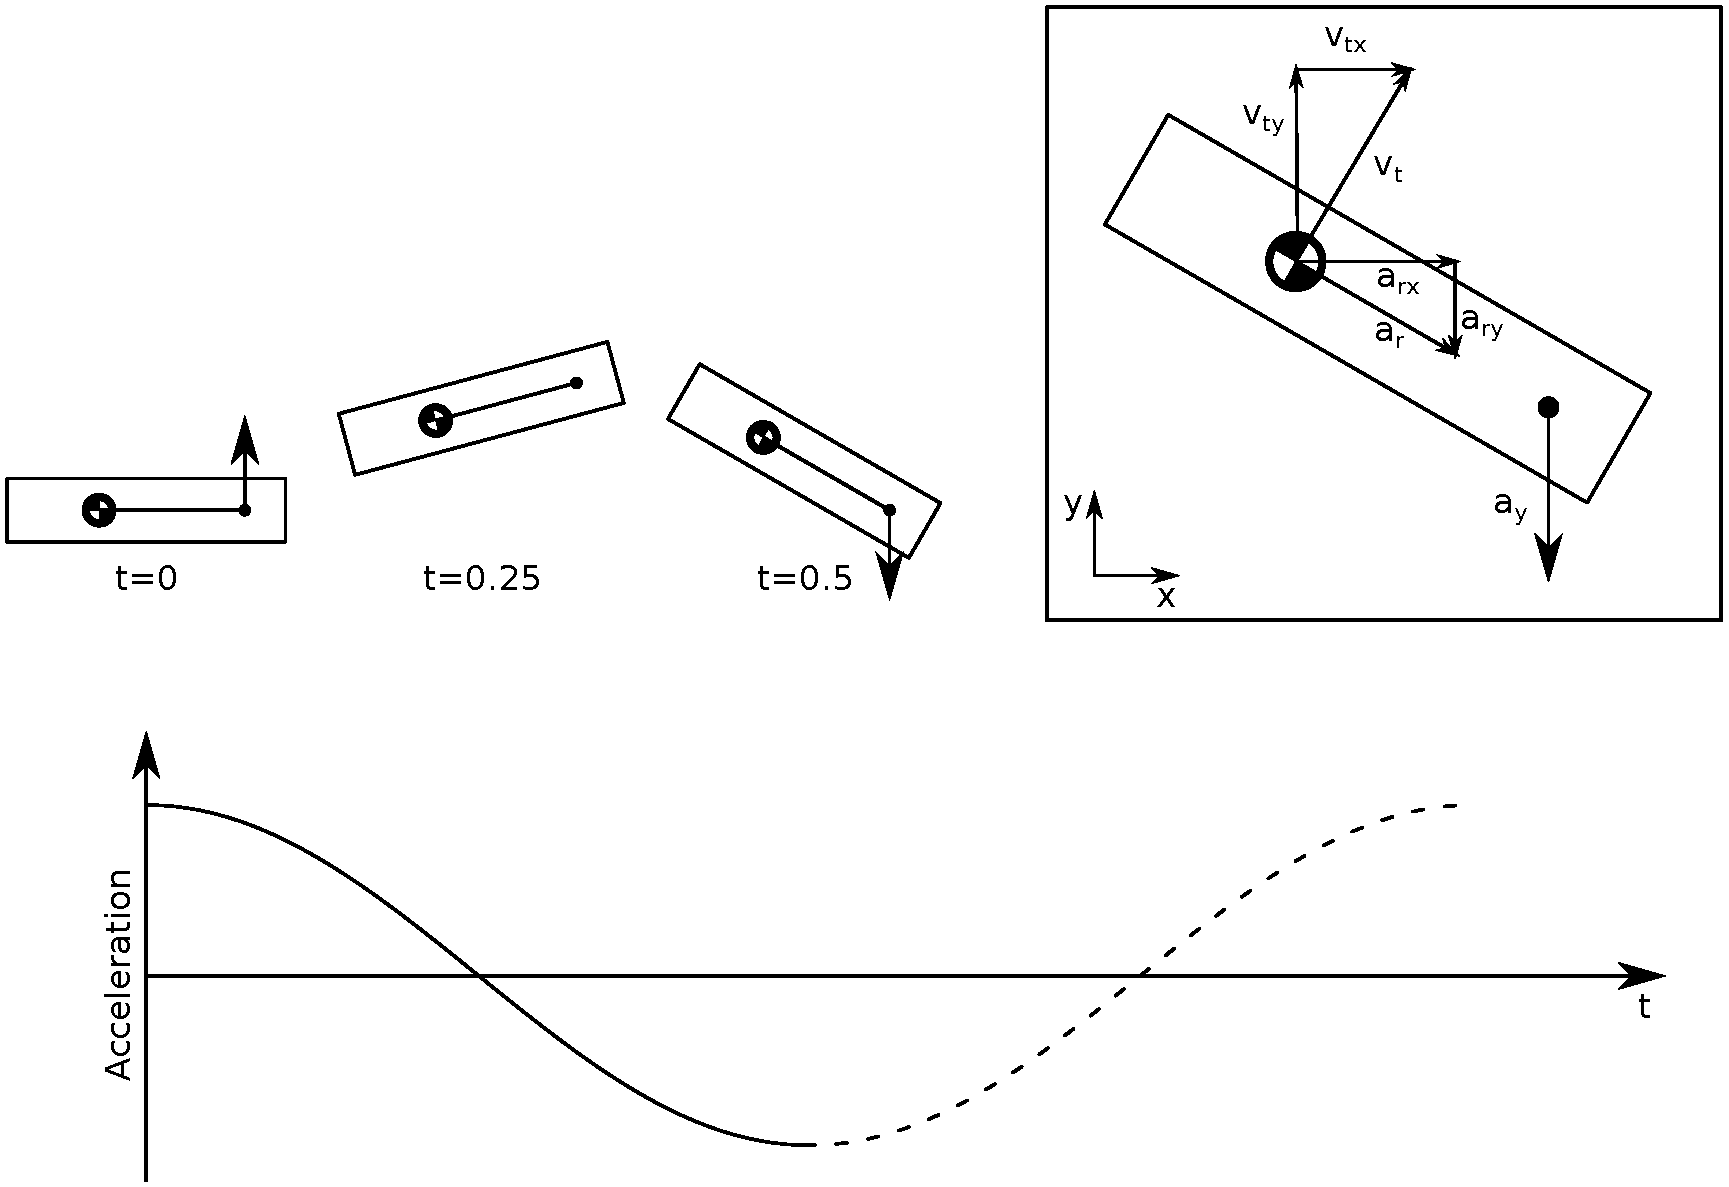
\includegraphics[width=0.7\linewidth]{manuscript/figures/kinematics.pdf}
    \caption{Simplified kinematics of an eccentric mass undergoing harmonic oscillations.}
    \label{fig:kinematics}
\end{figure}

The paper is subdivided into four sections: first, a table-top experiment (\autoref{sec:experiment}) is shown, capable of reproducing the torsional coupling. A section on finite-element-simulations (\autoref{sec:simulations}) follows. Finally, a discrete system of differential equations (\autoref{sec:3dof}) is presented. The final section (\autoref{sec:discussion}) discusses the shortcomings of the previously presented approaches and discusses implications for future research into the topic. 

\clearpage

\section{Cantilever experiment}
\label{sec:experiment}

As a first proof of concept, we built a table-top experiment that allows us to demonstrate the effect of an eccentric mass on the vibrations of a cantilevered beam. As a beam, we chose a wooden rod (massive beech, 0.006 m diameter) with a free length of 0.7 m. At the free end of the rod, we placed a 3D-printed lever that allowed us to add M8 bolts (0.028 m length, 0.0129 kg) to control eccentric mass. Lever length was 0.082 m weighing a total of XX kg. A second rod made of fibre glass (diameter 0.008 m) was placed next to the cantilevered beam. \autoref{fig:setup} shows the experimental setup. The second rod was used to displace the cantilevered beam from its resting position  by pulling the cantilevered beam towards the second rod using a thin thread. Initial displacement at the top of the rod was 0.135 m and three different masses (no bolts, two bolts, four bolts) were tested in the experiment. To release the cantilevered beam from it displaced position, the thread was burned using a lighter. While this release mechanism seems somewhat archaic, it ensures that no external torque is added to the system upon release. For each mass, the experiment was repeated three times. A MEMS-based inertial measurement (MPU 9255, InvenSense TDK, Tokyo, Japan) unit placed on top of the cantilevered beam measured linear acceleration and angular velocity with a sampling rate of 100 Hz. Measurements were recorded using a Raspberry Pi 400 and a custom written python script. All raw data is available at zenodo. 

Results were post-processed using a Jupyter Notebook and Python3. The Jupyter Notebook is available here. 

\begin{figure}[ht!]
    \centering
    \includegraphics[width=0.5\linewidth]{manuscript/figures/setup.png}
    \caption{Experimental setup}
    \label{fig:setup}
\end{figure}

\clearpage

\textbf{ToDo}

\begin{itemize}
    \item Add time series to the section
    \item estimate damping
    \item add table with damping and stiffness for both linear motion and torsion
    \item normalize data with damping to estimate undamped system
    \item redo plots with proper axis etc
\end{itemize}

\begin{figure}
    \centering
    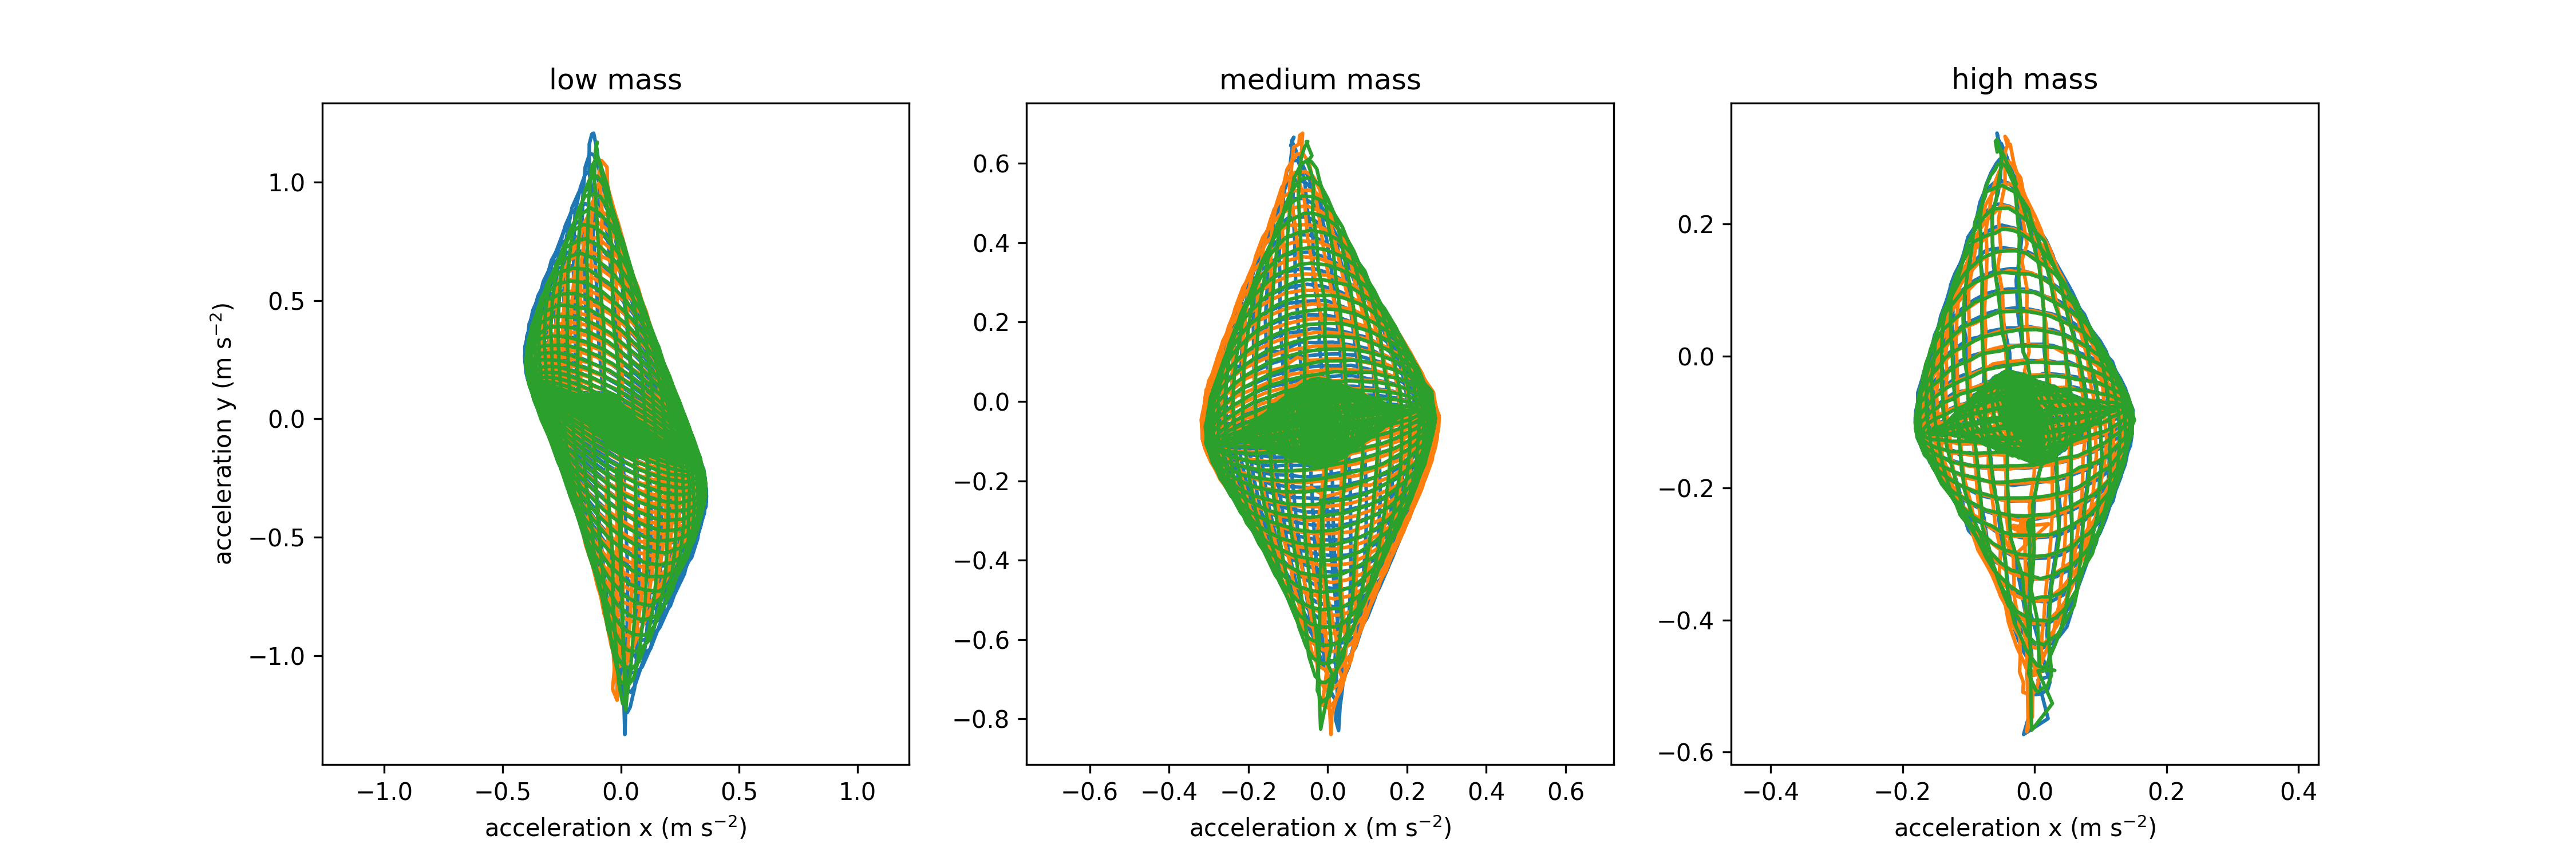
\includegraphics[width=\linewidth]{results/experiment/lissajous.png}
    \caption{Lissajous figures (orbits) for three different eccentric masses. \andy{[What are top's masses and moment of inertias of these configurations?]}}
    \label{fig:lissajous}
\end{figure}

\begin{figure}
    \centering
    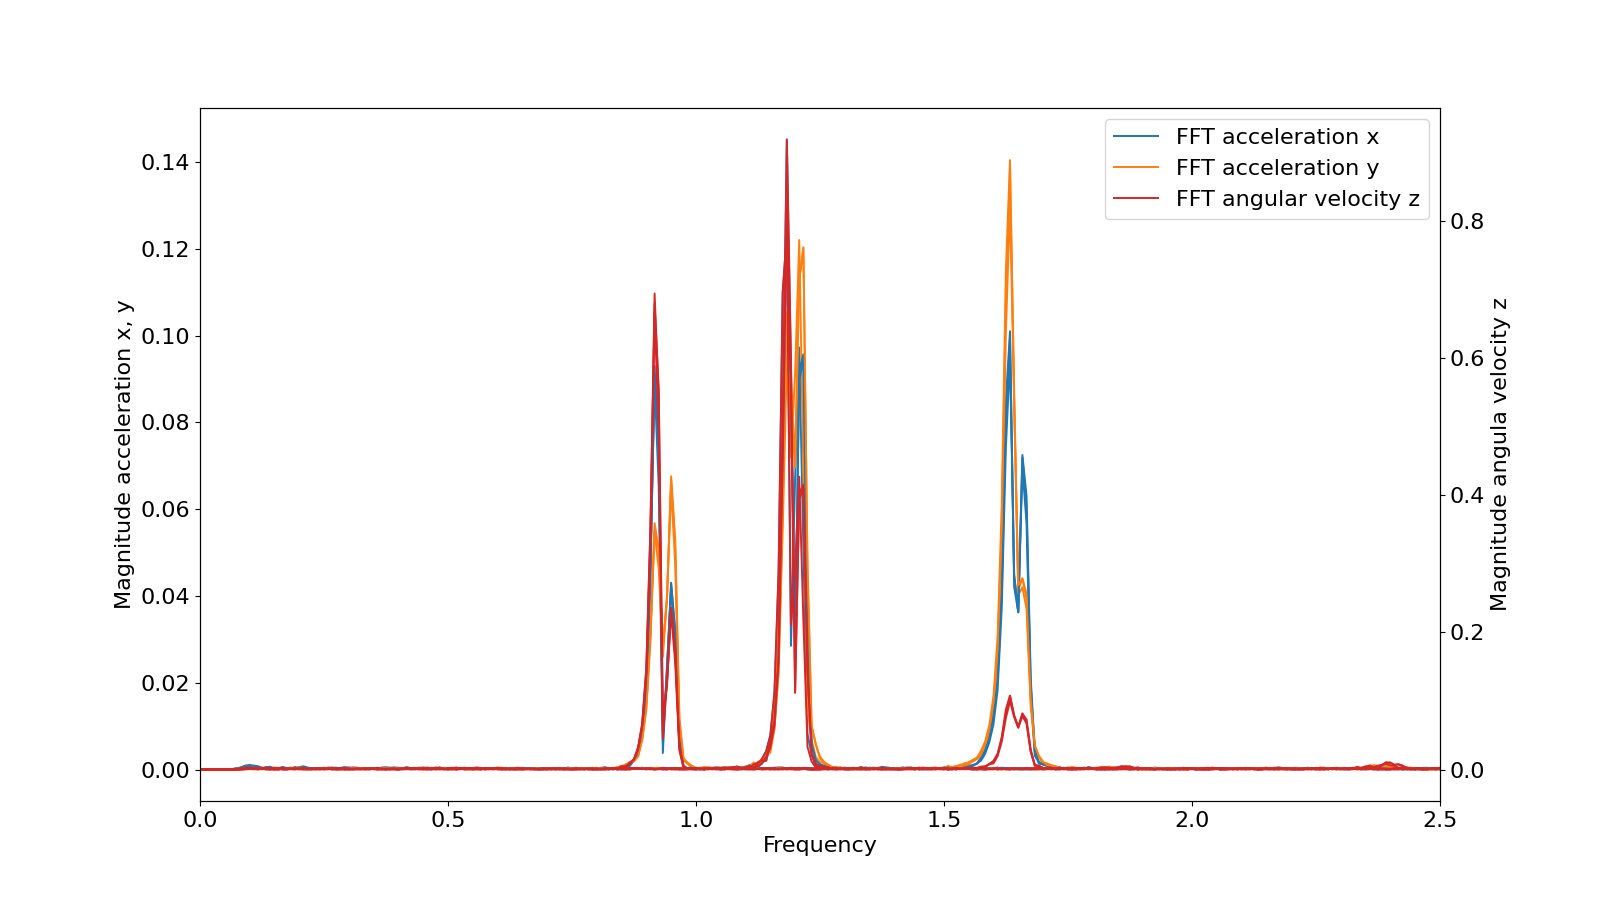
\includegraphics[width=\linewidth]{results/experiment/spectrum.png}
    \caption{Caption}
    \label{fig:spectrum}
\end{figure}

\clearpage

\section{Simulations (BAS)}
\label{sec:simulations}

\subsection{Simulation Setup}

\paragraph{Model}
A structural model was built to represent the simplified system as shown in Figure \ref{fig:loading}. The support structure was modelled with on linear one-dimensional finite element equations for tension, torsion and bending. Homogeneous linear elastic material was assumed and Euler Bernoulli beam theory was used for bending. It is assumed damping does not affect the formation of orbital motion and is thereby neglected, and thus the model can be described by \( \mathbf{M}\ddot{\mathbf{u}}+\mathbf{K}\mathbf{u} = \mathbf{F} \).
The support structure is modelled as a vertical cylinder with constant cross-section. The foundation is modelled by six springs, one spring for each degree of freedom of the system. The eccentric mass is modelled as a cube with distributed mass, without eccentricity, and an additional eccentric point mass. The eccentricity and related coupling of the point mass is linearised and considered in the horizontal plane only (rotation about vertical axis), since for tower top motions of offshore wind turbines rotation about horizontal axes is assumed negligible. The resulting mass matrix for the distributed mass and eccentric point mass, added to the top node of the structural model, is presented below.
% \begin{equation}
%     M = 
% \end{equation}
\begin{enumerate}
    \item add mass matrix
\end{enumerate}

\paragraph{Loads}
For the simulations, initial deformation and static load due to dead-weight were considered. No dynamic forces were applied. Initial deformations for two cases were obtained by applying force in the horizontal plane at the centre of the top of the model, with an angle of 90 degree and 85 degree witch respect to the eccentricity of the point mass. For each force orientation, a simulation with and simulation without gravity was done. 


\subsection{Simulation Results}



\clearpage

\section{A vibration model with three degrees of freedom}
\label{sec:3dof}

A common approach to study vibrations is to reduce the real system into a simplified model that consists of discrete components. In this approach, one aims to describe the real system as simple as possible to generate the main dynamics of the real system. Many vibration phenomena can be sufficiently described with systems with only one or two degrees of freedom. Here, we present a model with three degrees of freedom that seems to capture the main dynamics of the real system.
\par 
We model the real system in two dimensions (\autoref{fig:3dof-system}). The tower's bending is modelled as a linear spring, which is connected to a fixed point, which represents the tower's foundation, and to a first body, which represents the tower's top section. The tower's torsion is modelled with a torsional spring that connects a second body with a fixed angle in the inertial reference frame. This second body is pinned to the first body such that it translates with the first body, but rotates freely. Consequently, the system's three degrees of freedom are: the first body's position in $x$ and $y$ direction and the second body's orientation.
\par 
By applying the physical laws of conservation of linear and angular momentum, we derived the equations of motions for the system (a derivation is available as supplemental material). The system's equations of motion read:
\begin{equation}
    (m_1 + m_2) \ddot{x} - \cos(\theta) m_2 d \ddot{\theta} + \sin(\theta) m_2 d \dot{\theta}^2 + k_1 x = 0,\label{eq:eom-x}
\end{equation}
\begin{equation}
    (m_1 + m_2) \ddot{y} - \sin(\theta) m_2 d \ddot{\theta} - \cos(\theta) m_2 d \dot{\theta}^2 + k_1 y = 0,\label{eq:eom-y}
\end{equation}
\begin{equation}
    (I_{zz} + m_2 d^2)\ddot{\theta} - \cos(\theta) m_2 d \ddot{x} - \sin(\theta)m_2 d \ddot{y} + k_2 \theta = 0.\label{eq:eom-theta}
\end{equation}

The equations can be arranged to have only acceleration on the left hand side:
\begin{equation}
    \ddot{x} = \frac{1}{m_1 + m_2} \left( \cos(\theta) m_2 d \ddot{\theta} - \sin(\theta) m_2 d \dot{\theta}^2 - k_1 x \right),\label{eq:eom2-x}
\end{equation}
\begin{equation}
   \ddot{y} = \frac{1}{m_1 + m_2} \left(\sin(\theta) m_2 d \ddot{\theta} + \cos(\theta) m_2 d \dot{\theta}^2 - k_1 y \right),\label{eq:eom2-y}
\end{equation}
\begin{equation}
    \ddot{\theta} = \frac{1}{I_{zz} + m_2 d^2} \left(\cos(\theta) m_2 d \ddot{x} + \sin(\theta)m_2 d \ddot{y} - k_2 \theta \right) \label{eq:eom2-theta}
\end{equation}

Several terms couple translation ($x$ and $y$) with rotation ($\theta$): for example, the acceleration in the $x$ direction, $\ddot{x}$ is equal to terms that contain $\ddot{\theta}$ and $\dot{\theta}$ (\autoref{eq:eom2-x}). Such coupling terms are necssary to appear in the equation as otherwise only linear motion would be possible -- in other words, the mass would move back and forth on a straight line.
\par 
The translational acceleration is affected by the second mass' centrifugal and Euler forces. Centrifugal force acts in the $-\hat{r}$ direction and reads, 
\begin{equation}
    m_2 d \dot{\theta}^2,
\end{equation}
and Euler force acts in the $\hat{\theta}$ direction and reads
\begin{equation}
    m_2 d \ddot{\theta}.
\end{equation}
The equation for $\ddot{\theta}$ (\autoref{eq:eom2-theta}) was derived by applying conservation of angular momentum around the center of mass $G$. The force that acts at the location where the second body is pinned to the first body depend on the first body's acceleration in $x$ and $y$ direction such that there are also coupling terms with $\ddot{x}$ and $\ddot{y}$ in the equation for $\ddot{\theta}$  (\autoref{eq:eom2-theta}).
\par 
As expected, the equations also show that if $d=0$ the coupling terms disappear:
\begin{equation}
    (m_1 + m_2) \ddot{x} = - k_1 x,
\end{equation}
\begin{equation}
   (m_1 + m_2) \ddot{y} = - k_1 y,
\end{equation}
\begin{equation}
    I_{zz}\ddot{\theta} = - k_2 \theta.
\end{equation}

\begin{figure}
    \centering
    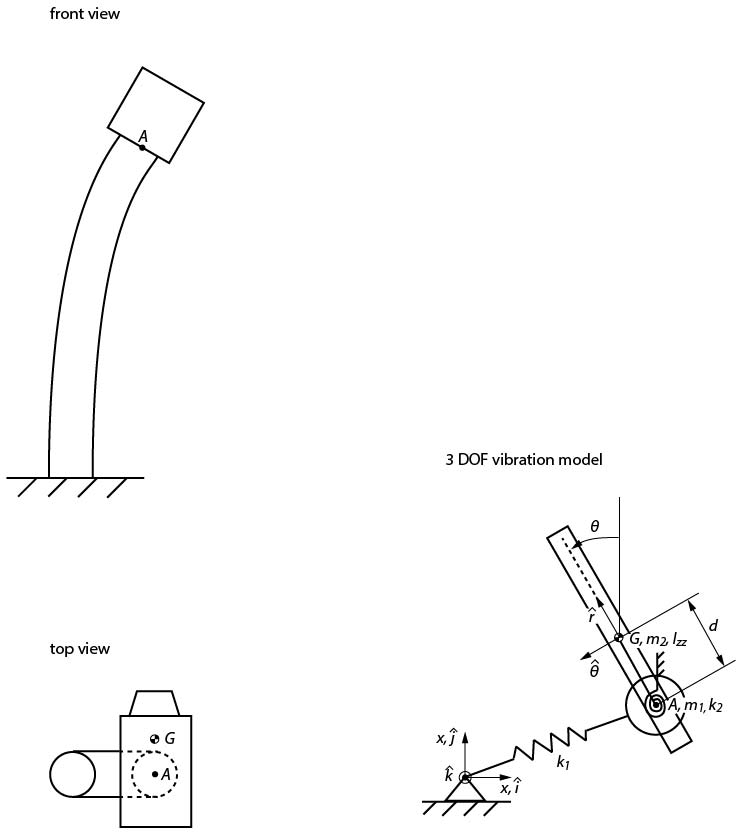
\includegraphics{manuscript/figures/vibration_model.jpg}
    \caption{A vibration model with three degrees of freedom (DOF).}
    \label{fig:3dof-system}
\end{figure}

The vibration model can reproduce the type of motions that were measured in the table top experiment and in the offshore measurement campaign [??? maybe the offshore measurements not]. \autoref{tab:3dof-variable-values} lists the parameter values that were estimated from the table top experiment and the offshore measurement campaign.

\begin{table}[]
    \centering
    \begin{tabular}{l l l l}
    \toprule
         Quantity & Table top experiment & Offshore measurements & Unit \\
         \midrule
         $m_1$ & 0.0093 & 320$\times$10$^3$ & kg\\ 
         $m_2$ & \{X, 0.044, X\} & 450$\times$10$^3$ & kg\\ 
         $k_1$ & 4.5 & 3.4$\times$10$^6$ & N\,m$^{-1}$ \\ 
         $k_2$ & 0.001 & 3.6$\times$10$^9$ & Nm\,deg$^{-1}$ \\ 
         $d$ & \{X, 0.038, X\} & 0.28 & m\\ 
         $I_{zz}$ & \{X, 5$\times$10$^{-5}$, X\} & 3.6$\times$10$^7$ & kg\,m$^2$ \\ 
         $\sqrt(x_0^2 + y_0^2)$ & 0.135 & - & m\\
         \bottomrule
    \end{tabular}
    \caption{Values used in the 3-DOF vibration model that correspond to the table top experiment and the offshore measurements.}
    \label{tab:3dof-variable-values}
\end{table}

\clearpage

\section{Discussion (ALL)}
\label{sec:discussion}

\begin{itemize}
    \item future work
    \item implications for offshore wind
\end{itemize}

\clearpage

\bibliographystyle{unsrtnat}
\bibliography{references}  %%% Uncomment this line and comment out the ``thebibliography'' section below to use the external .bib file (using bibtex) .


%%% Uncomment this section and comment out the \bibliography{references} line above to use inline references.
% \begin{thebibliography}{1}

% 	\bibitem{kour2014real}
% 	George Kour and Raid Saabne.
% 	\newblock Real-time segmentation of on-line handwritten arabic script.
% 	\newblock In {\em Frontiers in Handwriting Recognition (ICFHR), 2014 14th
% 			International Conference on}, pages 417--422. IEEE, 2014.

% 	\bibitem{kour2014fast}
% 	George Kour and Raid Saabne.
% 	\newblock Fast classification of handwritten on-line arabic characters.
% 	\newblock In {\em Soft Computing and Pattern Recognition (SoCPaR), 2014 6th
% 			International Conference of}, pages 312--318. IEEE, 2014.

% 	\bibitem{hadash2018estimate}
% 	Guy Hadash, Einat Kermany, Boaz Carmeli, Ofer Lavi, George Kour, and Alon
% 	Jacovi.
% 	\newblock Estimate and replace: A novel approach to integrating deep neural
% 	networks with existing applications.
% 	\newblock {\em arXiv preprint arXiv:1804.09028}, 2018.

% \end{thebibliography}


\end{document}
